%%%%%%%%%%%%%%%%%%%%%%%% ExtendedAbstract.tex %%%%%%%%%%%%%%%%%%%%%%%%
%                                                                    %
%  Template for the 10-page extended abstract to be submitted for    %
%  the MSc degree conferral at Instituto Superior Tecnico.           %
%                                                                    %
%  Author:                                                           %
%                                                                    %
%       Andre C. Marta                                               %
%       Area Cientifica de Mecanica Aplicada e Aeroespacial          %
%       Departamento de Engenharia Mecanica                          %
%       Instituto Superior Tecnico                                   %
%       Av. Rovisco Pais                                             %
%       1049-001 Lisboa                                              %
%       Portugal                                                     %
%       Tel: +351 21 841 9466                                        %
%                        3466 (extension)                            %
%       Email: andre.marta@ist.utl.pt                                %
%                                                                    %
%  Created:       Dec  2, 2011                                       %
%  Last Modified: Dec 27, 2011                                       %
%%%%%%%%%%%%%%%%%%%%%%%%%%%%%%%%%%%%%%%%%%%%%%%%%%%%%%%%%%%%%%%%%%%%%%
% This document uses the LaTeX class file "article.cls"              %
%%%%%%%%%%%%%%%%%%%%%%%%%%%%%%%%%%%%%%%%%%%%%%%%%%%%%%%%%%%%%%%%%%%%%%
\documentclass[8pt,a4paper,twocolumn]{article}

%%%%%%%%%%%%%%%%%%%%%%%%%%%%%%%%%%%%%%%%%%%%%%%%%%%%%%%%%%%%%%%%%%%%%%
% Document preamble
%%%%%%%%%%%%%%%%%%%%%%%%%%%%%%%%%%%%%%%%%%%%%%%%%%%%%%%%%%%%%%%%%%%%%%

%% Builds upon the graphics  package, providing a key-value interface
%% for optional arguments to the \includegraphics command that go far
%% beyone what the graphics package offers.
%% http://www.ctan.org/tex-archive/help/Catalogue/entries/graphicx.html
%% if you use PostScript figures in your article
%% use the graphics package for simple commands
%% \usepackage{graphics}
%% or use the graphicx package for more complicated commands
%% \usepackage{graphicx}
%% or use the epsfig package if you prefer to use the old commands
%% \usepackage{epsfig}
\usepackage{graphicx} % Enhanced LaTeX Graphics
\usepackage{siunitx}

%Tipo de letra Arial
\usepackage{helvet}
\renewcommand{\familydefault}{\sfdefault}

% acentos e cedilhas
\usepackage[utf8]{inputenc}
%\usepackage[T1]{fontenc}

% Multiple figures
%\usepackage{subfigure} % subcaptions for subfigures
%\usepackage{subfigmat} % matrices of similar subfigures

\usepackage[font=footnotesize, skip = 1pt, labelfont=bf]{caption}
\usepackage[font=footnotesize]{subcaption}

% Declaring new column types
% 'dcolumn' package defines D to be a column specifier with
% three arguments: D{<sep.tex>}{<sep.dvi>}{<decimal places>}
%                  D{<sep.tex>}{<sep.dvi>}{<left digit places>.<right digit places>}
\usepackage{dcolumn}           % decimal-aligned tabular math columns
% d takes a single argument specifying the number of decimal places, e.g., d{2}
% or the number of digits to the left and right of the seperator, e.g., d{3.2}
\newcolumntype{.}   {D{.}{.}{-1}} % column alignedd on the point separator '.'
\newcolumntype{d}[1]{D{.}{.}{#1}} % column centered on the point separator '.'
\newcolumntype{e}   {D{E}{E}{-1}} % column centered on the exponent 'E'
\newcolumntype{E}[1]{D{E}{E}{#1}} % column centered on the exponent 'E'

%% American Mathematical Society (AMS) plain Tex macros
%%
%% The amsmath package is the principal package in the AMS-LaTeX distribution
%% http://www.ctan.org/tex-archive/help/Catalogue/entries/amsmath.html
\usepackage{amsmath}
\DeclareMathSizes{7}{7}{3}{3} 
\usepackage{pifont}
%%
%% The amsfonts package provides extended TeX fonts
%% http://www.ctan.org/tex-archive/help/Catalogue/entries/amsfonts.html
\usepackage{amsfonts}
%% The amssymb package provides various useful mathematical symbols
\usepackage{amssymb}
%%
%% The amsthm package provides extended theorem environments
%% http://www.ctan.org/tex-archive/help/Catalogue/entries/amsthm.html
\usepackage{amsthm}

%% Improves the interface for defining floating objects such as figures and tables.
%% The package also provides the H float modifier option of the obsolete here package.
%% http://www.ctan.org/tex-archive/help/Catalogue/entries/float.html
\usepackage{float}

%% Control sectional headers. 
%% http://www.ctan.org/tex-archive/help/Catalogue/entries/sectsty.html
\usepackage{sectsty}
%%
%% Redefine the font size of the 'section' and 'subsection' headings
\newcommand{\myFontSize}{\fontsize{9}{0}\selectfont}
\sectionfont{\myFontSize}       % 10pt, Bold face (default)
\subsectionfont{\myFontSize} % 10pt, Plain face

%% Select alternative section titles.
%% http://www.ctan.org/tex-archive/help/Catalogue/entries/titlesec.html
\usepackage{titlesec}
\usepackage{booktabs}
%\usepackage{multirow}
%\usepackage{array}
\usepackage{csquotes}% Recommended
%\usepackage[style=authoryear, backend=bibtex, doi=false,isbn=false,url=false,eprint=false,dashed=false,maxcitenames=2, maxbibnames=100]{biblatex}
%\addbibresource{library.bib}

%%
%% Left indent, before and after spacing
%% (The starred version kills the indentation of the paragraph following the title)
\titlespacing*{\section}{0pt}{10pt}{0pt}
\titlespacing*{\subsection}{0pt}{10pt}{0pt}

%% Section numbers with trailing dots. 
%% http://www.ctan.org/tex-archive/help/Catalogue/entries/secdot.html
\usepackage{secdot}
\usepackage{epstopdf}
%%
%% Also put a dot after the subsection number
\sectiondot{subsection}
%% Set a space between dot and heading text
\sectionpunct{section}{. }    % By default, \sectiondot places a \quad
\sectionpunct{subsection}{. } % after the number

% These are exact settings for a A4 page with top margin of
% 25 mm, bottom margin of 30 mm, left and right margins of 25 mm,
% printable area 242 X 160 mm.

\setlength{\topmargin}{-10.4mm}
\setlength{\headheight}{0.0mm}
\setlength{\headsep}{10.0mm}
\setlength{\textwidth}{160mm}
\setlength{\textheight}{242mm}
\setlength{\oddsidemargin}{0mm}
\setlength{\evensidemargin}{0mm}
\setlength{\marginparwidth}{0mm}
\setlength{\marginparsep}{0mm}

% New command to refer to equations as Eq.(1),Eq.(2),...
\newcommand{\eqnref}[1]{Eq.(\ref{#1})}

%%%%%%%%%%%%%%%%%%%%%%%%%%%%%%%%%%%%%%%%%%%%%%%%%%%%%%%%%%%%%%%%%%%%%%%%%%%%%%%%%%%%%%%%
% Title, authors and addresses

\title{\bfseries LINA: A Serious Game To Help Children Improve Social Relations With Their Peers}
\date{July 2019}
\author{Diogo Martins \\ diogo.f.martins@tecnico.ulisboa.pt \\ \\ Instituto Superior Técnico, Lisboa, Portugal}

%%%%%%%%%%%%%%%%%%%%%%%%%%%%%%%%%%%%%%%%%%%%%%%%%%%%%%%%%%%%%%%%%%%%%%%%%%%%%%%%%%%%%%%%
\begin{document}

% Begin one column section for title and abstract
%
% http://www.faqs.org/faqs/de-tex-faq/part5/
\twocolumn[
\begin{@twocolumnfalse}
\maketitle

	%%%%%%%%%%%%%%%%%%%%%%%%%%%%%%%%%%%%%%%%%%%%%%%%%%%%%%%%%%%%%%%%%%%%%%
%     File: ExtendedAbstract_abstr.tex                               %
%     Tex Master: ExtendedAbstract.tex                               %
%                                                                    %
%     Author: Andre Calado Marta                                     %
%     Last modified : 2 Dez 2011                                     %
%%%%%%%%%%%%%%%%%%%%%%%%%%%%%%%%%%%%%%%%%%%%%%%%%%%%%%%%%%%%%%%%%%%%%%
% The abstract of should have less than 500 words.
% The keywords should be typed here (three to five keywords).
%%%%%%%%%%%%%%%%%%%%%%%%%%%%%%%%%%%%%%%%%%%%%%%%%%%%%%%%%%%%%%%%%%%%%%

%%
%% Abstract
%%
\begin{abstract}

Children that have problems in developing socialization before his teens can become socially isolated, leading to low self-esteem and social alienation, and possibly snowballing into more serious psychological problems further into adulthood. In this document we present a proposal and implementation for a Serious Game, LINA, that uses Contact Theory to help pre-adolescent children improving the relations with their peers. In LINA, the players, children from 10 to 12 years old, will try to find out what happened to a missing colleague - Lina - and her story through the discovery of augmented reality clues and overcoming challenges cooperatively. This document specifies the game concept, methodology and implementation of a digital prototype for demonstration. Also evaluates said prototype regarding its usability, enjoyment and interest for the players. Conducted evaluation determined that the players find the gameplay and story fun and are keen on playing more of the game. Future work involves revising this first prototype with the feedback from the evaluation session, coming up with new challenges and exploring technical limitations of Augmented Reality in the game context.

%%
%% Keywords (max 5)
%%
\noindent{{\bf Keywords:}} Augmented Reality; Contact Theory; Serious Game; User-Centered Design.
\end{abstract}



\end{@twocolumnfalse}
]
	\section{Introduction}
\label{sec:intro}

\begin{quotation}
``Man is by nature a social animal; an individual who is unsocial naturally and not accidentally is either beneath our notice or more than human. Society is something that precedes the individual. Anyone who either cannot lead the common life or is so self-sufficient as not to need to, and therefore does not partake of society, is either a beast or a god."
\par - Aristotle.
\end{quotation}

% #############################################################################
\par Nowadays, contact between individuals is increasingly made through digital means: Instant messengers, Voice-over-IP and video calls. Technology allows us to be closer to people, even when they are across the globe. People that do not know each other are brought closer and form social relationships thanks to that same technology. And one particular situation is the approximation of individuals through video games. For example, studies have shown that cooperative video games can bring families closer \cite{wang_taylor_sun_2018} and improve the social and affective aspects of hospitalized children by having interactions through a video game context with other children in the same condition \cite{gonzalez-gonzalez_toledo-delgado_collazos-ordonez_gonzalez-sanchez_2014}. 

\subsection{Problem}
\par Socialization is a key process in the psychological development of a child. As the child gradually becomes a teen, his/her \textbf{social cognition} mastery starts to expand and his/her awareness towards the social environment around him/her increases steadily. Enthusiast, cooperative and responsive children are usually seen as the more popular in his group of people, and children lacking social interactions, or that feel vulnerable by their psycho-social development and isolate themselves, more often will be deemed less popular and this can generate anxiety and will diminish their self-esteem \cite{tavares_pereira_gomes_monteiro_gomes_2007} \cite{campos_1990} creating a snowball into social alienation. So, a child/pre-adolescent that has isolated himself, either by unconscious self-imposition or due to reasons external to him, has diminished social capabilities and lacks will-power and/or opportunities to engage in social activities with others. 

\par \textbf{How can we help improve pre-adolescents' abilities to establish successful relations with their peers?} To address this issue we explore the use of a Serious Game, but given the complexity of the problem, both in terms of development and evaluation, we will start with a first step in this direction by focusing on how to create such game. \textbf{How can we make such Serious Game fun, enjoyable, and easy to use for children?}


%##############################################################################
\subsection{Approach}

\par We present a proposal and implementation for a serious game, LINA, with a very strong social component that aims to help children improve relations with their peers. In LINA, the players, children from 10 to 12 years old, will try to find out what happened to a missing colleague - Lina - and her story through the discovery of clues and surpassing challenges.
\par There are three concept pillars used in the concept described above: Contact Theory, Augmented Reality and User-Centered Design. Contact Theory tries to end negative conceptions about intergroup peers. We will be applying Contact Theory when trying to get the children to cooperate to achieve a common goal: finding out what happened to Lina. To do so, they will need to complete challenges as a group, by socializing with each other, thereby trying to improve their relationships, and hopefully creating new ones. 
\par Augmented Reality is not a new technology employed in the videogame industry. Recently, it has found enormous popularity with the worldwide-phenomenon that was \textit{Pokémon Go}. Tateno et al. have inclusively written about the hypothesis that the videogame could help children and teens with severe social withdrawal, although studies were not made to support the claim.\cite{tateno_skokauskas_kato_teo_guerrero_2016}
\par As this project will be targeting pre-adolescent children, special care must be considered when designing the concept prototype, as one of our objectives is trying to create a game that children won't find difficult to use. A clean, unambiguous interface with established conventions (like using well-know metaphors for buttons) and restricted freedom makes the users' choice-making clearer and streamlined. However, such concept is bound to iterative revisions to improve the users' interaction.

	% A Theory section should extend, not repeat, the background to the
% article already dealt with in the Introduction and lay the
% foundation for further work.

\section{Background}
\label{sec: backg}

\subsection{Contact Theory}
\par Before Allport hypothesized the ``Intergroup Contact Hypothesis" in 1954, it was believed that inter-group contact would inevitably lead to conflict, result from nineteenth century Social Darwinism, where most groups felt superior to others, naturally leading to hostility. However, no studies were conducted at that time and therefore no empirical evidence was found to support the claim. \cite{pettigrew_1998} 
\par Allport, in \textit{The Nature of Prejudice (1954)}, after extensive study, would lately adapt these four conditions into four ``positive factors" that need to be present to reduce prejudice:

\begin{enumerate}
\item \textbf{Equal status between groups.} This equal status that Allport states refers \textbf{within} the situation, not \textbf{coming into}. Some writers defend that should be of equal status prior to entering the situation, but research has shown that equal status \textit{within} is enough and even more important than outside status.
\item \textbf{Common goals.} To reduce prejudice, active inter-group contact must share a common goal. By having the same objectives, the team constituents work effectively, harder and unitedly, as the different groups rely on each other, to accomplish it.
\item \textbf{Inter-group cooperation.} To work in unity towards the common goal, logically, there must not be group competition. Cooperation should be independently emphasized to each subject, as the feeling of competition undermines the effort made by the rest of the team.
\item \textbf{Support of authorities, law or custom.} With a climate of support surrounding the contact's environment, inter-group contact is more readily accepted and has more positive results. Field research in the military, business and religious institutions has emphasized the importance in support by the authority, as it is that authority that establishes the norms of acceptance.
\end{enumerate}

% #############################################################################
\subsection{Augmented Reality}
\par A variation of Virtual Reality, but different enough to warrant a distinction, the term ``Augmented Reality" has been around since the early 1990s. While the former focuses on creating a separate environment from the user point-of-view, isolating him from his ``real" environment, either through visual output, sounds, smells, or even tact, the last tries to enhance the current environment where the user is present, usually capturing it with a camera and overlaying it with information (e.g. text, images) but nevertheless still allowing the user to access the original information captured by his bio-sensors, i.e., eyes, ears, hence ``augmenting" his senses. \cite{sutherland_1968}
\par Azuma describes Augmented Reality as systems that: \cite{azuma_1997}
\begin{itemize}
    \item Combine real and virtual;
    \item Are interactive in real time;
    \item Are registered in three dimensions;
\end{itemize}

\par Augmented Reality has since gained popularity in the game community with the release of PokémonGO. In their work Das et al. hypothesize that Augmented Reality could have a social impact that is not normally associated but is inherent to the genre. Das et al. state that "in comparison to traditional video games, ARGs may be inherently more social.  Players are required to interact with the surroundings and often encounter friends and fellow players. For example, Pokémon GO and other ARGs have many features that promote social interaction between players. (...) Players on the same team are encouraged to work together to strengthen their Pokémon and gain or maintain control of PokéGyms. The team feature further increases the social component of Pokémon  GO  because  players  must  work  with  teammates  in  order  to  advance. " \cite{das_zhu_mclaughlin_bilgrami_milanaik_2017} This is an important foundation because it comes close to what we want to do with LINA, not exactly with the gym or Pokémon mechanic, but more on the part of using Augmented Reality to socialize and advance on the game. 


%####################################################################
\subsection{User-Centered Design}
\par User-Centered Design, is a broad term to describe design processes in which the users affect the development decisions. There are several ways the users can be involved: from requirements gathering and usability testing, to being made partners to designers through the design process.\cite{Abras04user-centereddesign} The term was coined by Donald Norman in his research laboratory in the University of California San Diego, but the concept was formed in his book \textit{The Psychology Of Everyday Things} (1988), where he states four rules for a design to be user-driven:
\begin{itemize}
    \item Make it easy to determine what actions are possible at any moment.
    \item Make things visible, including the conceptual model of the system, alternative actions, and the results of actions. 
    \item Make it easy to evaluate the current state of the system.
    \item Follow natural mappings between intentions and the required actions; between actions and the resulting effect; and between the information that is visible and the interpretation of the system state.
\end{itemize}
\par But for Norman just saying a design should be intuitive is not enough, so he states how important it is to consider some additional design principles to facilitate the designer and the user:
\begin{enumerate}
    \item Simplify the structure of tasks. Make sure not to overload the users' short- and long-term memories. On average the user is able to remember five things at a time. For example, making a long sequence of menus would be counter-productive for a given task. 
    \item Make sure the task in consistent and provide mental aids for easy retrieval of information from long-term memory. Make sure the user has control over the task. 
    \item Make things visible: bridge the gulfs of Execution and Evaluation. The user should be able to figure out the use of an object by seeing the right buttons or devices for executing an operation. Trying to keep the menus as simple as possible while giving the options necessary, and only those, is a correct implementation of this principle.
\end{enumerate} 



	\section{Solution}
\label{sec: Methodology}
\par \textit{"Lina, your colleague and friend, did not appear today in class and your teacher knows that she will not come to school anymore, but does not know why. Although she sees your messages, does not answer them, she just sends an enigmatic image that appears to be on your desk. What could that mean?"}
\par With the first paragraph as premise, LINA is a mobile Augmented Reality videogame inserted in the D.O.T. - Die Offene Tür project \cite{dot_project_website_2017}, aiming towards "improving social connectedness through digital experiences". LINA aims to create an immersive experience, where the players take on the role of students in a class and engage with each other, guided by the game. This allows the players to socially connect themselves free of prejudice, acting as a field-levelling tool by providing them with an isolated fictional environment and by portraying (and socializing as those) fictional characters. Having begun focusing on the COPMI - Children of Parents with Mental Illness - the game has now broaden its target group to all children in the middle school ages (10-12 year olds) as they can also benefit from the fictional space that the game creates, as prejudice is not exclusive to children with special needs.

\begin{figure}
	\centering
	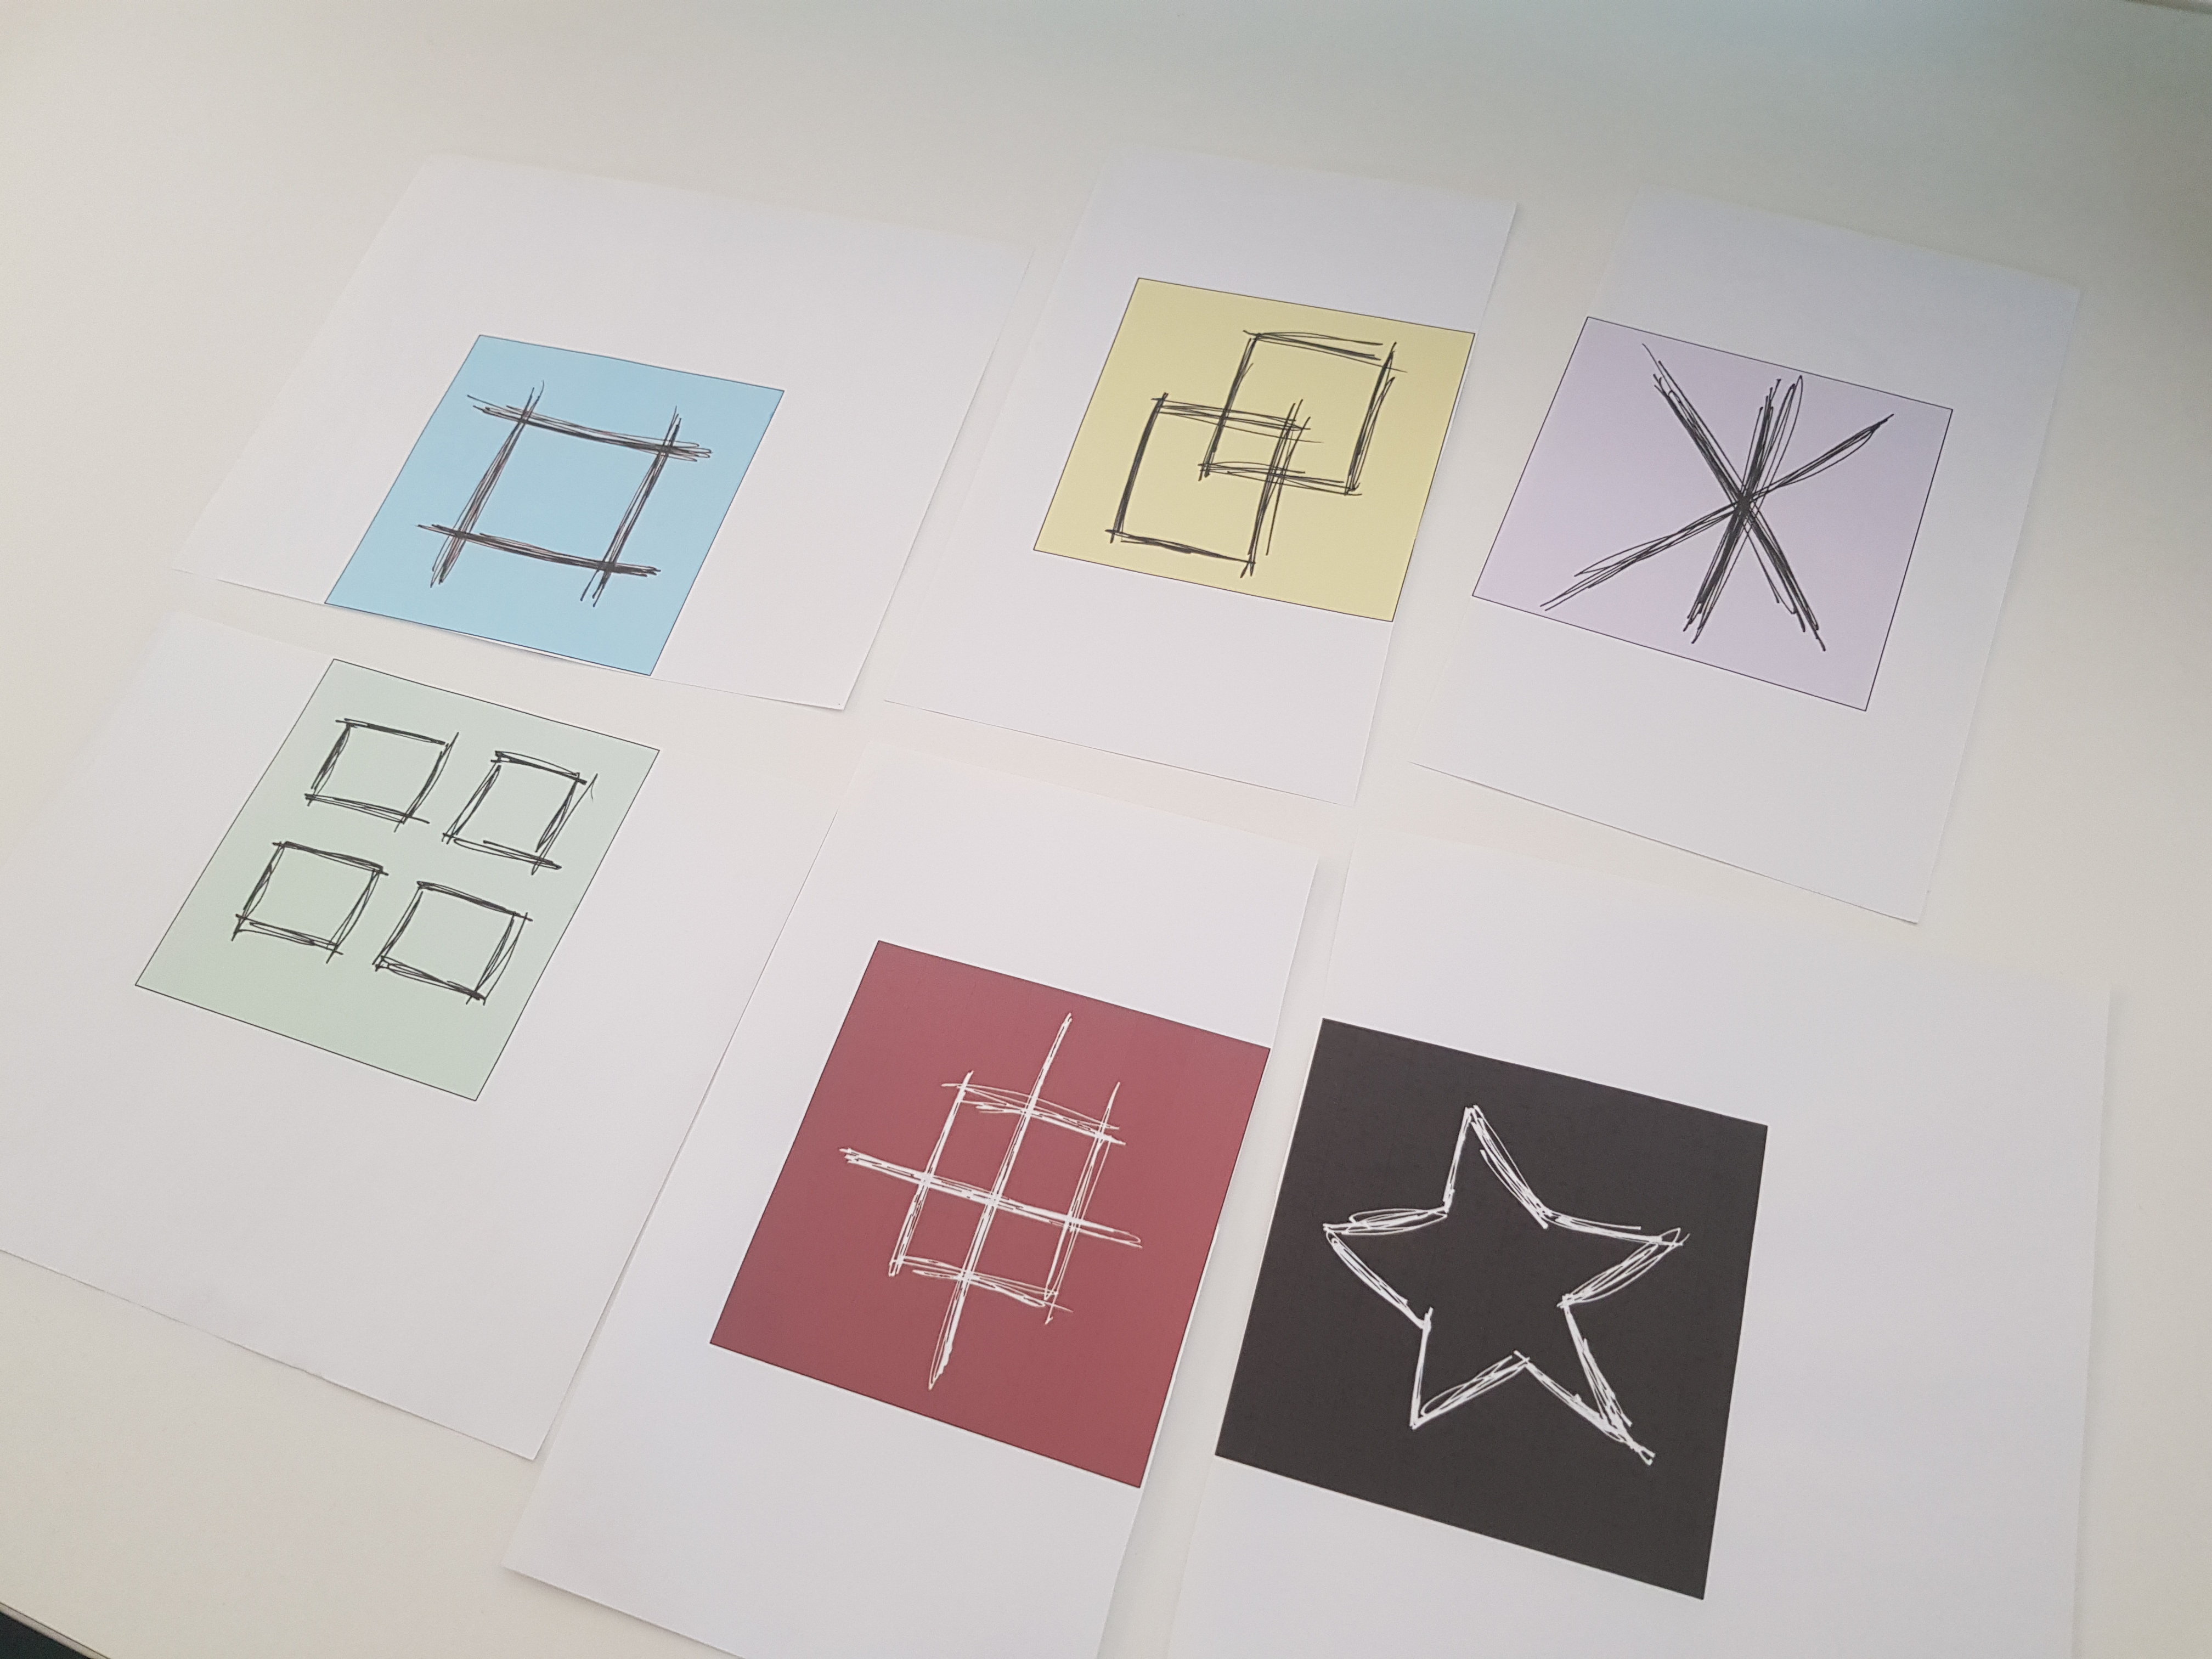
\includegraphics[scale = 0.05]{newIcons.jpg}
	\caption{The markers that are to be recognized and overlayed through Augmented Reality.}
	\label{fig:icons}
\end{figure}



\subsection{Concept} The basic concept of LINA is the search for a clue through the use of overlayed augmented reality over a marker. When scanning an image [Fig. \ref{fig:icons}] with the device's camera, an overlayed clue (usually an object that the player can interact with) is revealed, usually describing an important event involving Lina, followed with instructions to search for another image.
\par After the player completing 1 or 2 "stages", they must find another player - or group of players, henceforth designated as element - and solve a challenge presented to them. These challenges could be answering questions about the parts of story that only the other player knows about (which forces them into socializing when sharing their parts of the story), or having both elements perform a task together, for example simultaneously scanning a set of markers. This way the game creates an interesting way of socializing while at the same time exploring a narrative that relates to social isolation. This gives us the four ``positive factors" mentioned in Contact Theory:
\begin{itemize}
	\item Equal status between groups - All children will have the same importance in the game, all have important information that need to be shared among the others so that they can all advance in the narrative;
	\item Common goals - The shared goal is to overcome challenges and finish the game and find what happened to Lina.
	\item Inter-group cooperation - Only by sharing the information, or completing challenges together can they advance in the narrative, so there must be cooperation among themselves.
	\item Support of authorities, law or custom - The teacher, being the authority figure in the classroom, has given the explicit approval and is even directly involved in the game.
\end{itemize}
These ``stages" are not the same for all players: different players would get different stages so that they would get different pieces of the puzzle.
\par As the complexity of the game increases due to the elements scaling, multiple approaches have been discussed regarding the game's structure. Originally, each student started on his own and slowly paired up with his colleagues until the whole group searched for the final clue as one, like a perfect binary tree, with each node being an element: a leaf node representing a student, a non-leaf node representing a pairing and the root node the whole class. This structure would only work if the number of students in the class was a power of two, or else a student would have to either play alone while others were already paired, or skip stages to pair with a larger group, which would be unbalanced. Plus, the number of stages could be inappropriate to accommodate the number of students in class. 
\par Then it was considered to split the class in smaller groups of students, with each group playing LINA separately instead of being a single class, but that would defeat the purpose of pairing the children with someone that they get along with, plus it doesn't address the issue with the previous strategy.
\par Then it was concluded that instead of trying to make the number of stages according to the number of players, it should be the opposite: establish a fixed number of stages and split the class accordingly into groups of a pre-established size. For example, if a certain challenge needs elements of 4 or 5 persons then in a class of 9 it would split into [4,5], in a class of 18: [4,4,5,5], in a class of 23: [4,5,5,5,4]. Then at the end of the challenge the next elements are reshuffled (or perhaps the system could know which colleagues the player hasn't been paired with - needs further discussion) However it is necessary to first know how many stages LINA has before starting to split the class into groups, and then make the challenges flexible to accommodate groups of N or N+1.


\subsection{Structure, Challenges \& Story}
\par Presently, it has been discussed splitting LINA in sessions (or "episodes"): 5-10 minutes of recap in the beginning; 30-35 minutes of gameplay, where the children play some stages, initially by themselves, later in groups; and 10-15 minutes of discussion afterwards. 
\par A stage is the basic gameplay unit, similar to a level. There are 5 core stage archetypes in LINA:
\begin{enumerate}
	\item A roleplay-style stage, where the players are instructed to say something, or act in a certain way;
	\item A narrative-related stage, where the player only needs to pay attention to the narration or to the text presented to him in his screen;
	\item A simple find-the-marker stage where the player is tasked to find a marker, then has to interact with an object and finally gets a piece of information that either develops Lina's character or his character. 
	\item A find-the-marker stage that differs from the previous archetype when the information or objects gathered in this stage is going to be useful in a cooperation stage later on.
	\item And a cooperation stage where the players need to work together to complete a challenge. This relates with Contact Theory, where each player has the same importance in working towards the common goal.
\end{enumerate}

\par So far there are 7 different stages in the game:
\begin{itemize}
	\item Stage 1 - Registration and Initial Briefing: 
	\par An example of the first archetype, in this stage the students and the teacher engage in a role-playing scene where the teacher is making the presence list, with each student answering his/her (character's) name, and by failing to call Lina the class gets intrigued with her absence, moving on to the next stage.
	
	\item Stage 2 - \textit{Lina's Message}: 
	\par An example of the 2nd archetype, in this scene the player's character wonders how strange it is that Lina did not show up for class. He thinks to himself whether he should text Lina. After texting Lina asking what happened to her, she only answers back with a mysterious image. "What does that mean?" the player's character wonders. This prompts the player to search for this picture and thus setting up the premise for the first mission. As each player is going to search for a different image, the received image is going to be different for each player, making the number of different markers varying with the number of students in class.
	
	\item Stage 3 - \textit{Tutorial}: 
	\par \textit{Tutorial} is an example of the 3rd archetype, the first mission and entry point for the player into the proper game. After receiving the mysterious image from Lina's message, the player needs to find what it means. The markers will be placed directly on the player's desk, just to introduce them to the core mechanics of the game, like scanning and tapping the marker.
	
	\item Stage 4 - \textit{The Party and The Note}/\textit{The Picture On The Wall}: 
	\par This stage is another example of the 3rd archetype. In \textit{The Party and The Note} the player finds a crumpled-up paper that unravels a note that reveals that Lina didn't want to go to a colleague's birthday party. \par While one player is playing \textit{The Party and The Note}, another player is playing \textit{The Picture On The Wall}. In it he finds, upon scanning the marker, that art is Lina's best subject and that, when asked to draw someone that inspires her, she the drew the back of a hoodie.  \par \textit{The Picture On The Wall} was an idea from the original proof-of-concept where the students would have several drawings shown on a wall in real life, with a marker replacing Lina's drawing, prompting the students to scan the marker to see it the drawing, and make it as seamless as possible.
	
	\item Stage 5 - \textit{The Broken Screen}/\textit{The Broken Screen - Lina's PoV}: 
	\par Like Stage 4, \textit{The Broken Screen} and \textit{The Broken Screen - Lina's PoV} are two missions played in parallel by different players, that differ from the previous ones as they are setting up the cooperation stage that follows, falling under the 4th archetype. \par In \textit{The Broken Screen} the player finds a folder containing a letter from the teacher, Mr.Gordon, to the headmaster explaining how he found Lina and Ashley standing next to a broken computer. Lina first says that she and Ashley were the culprits but later she confesses to Mr.Gordon to have done it by herself.
	\par In \textit{The Broken Screen - Lina's PoV} the other player finds a note inside a backpack that reveals that Lina did not break the screen but it was in fact two older kids that bullied her into confessing the misdeed, and that Lina will correct things up, but did not say how.
	
	\item Stage 6 - \textit{Cooperative Question}: 
	\par When scanning the marker, the player finds an instruction telling to wait for the other player. When both players are at the marker they are asked to answer a question about the other player's part of \textit{The Broken Screen} story, which prompts the players into sharing their parts so they can answer the questions. When they correctly answer the question they unlock an instruction to find the next marker. This stage is an example of the 5th archetype.

    
	
	\item Stage 7 - \textit{Lina's Diary and Puzzle} - Archetypes 4 and 5:
	\par After unlocking the next marker in the challenge the players must find as a pair. When scanning the marker each player gets a different half of a page of Lina's diary. They are taken to a screen with four different images. The images are the same for both players, but their order differs. They are then instructed to tap on the images by the order they see on the other player's device. When they do so correctly both parts of the page unite to become a single page. One of the players is then asked to read Lina's diary to the other. This stage is a combination of archetypes 4 and 5 since there is a marker to be found but also a challenge after finding the marker, but does not make sense splitting into two different stages. 
	
	
\end{itemize}

\par It is necessary to reiterate that this project is still more than a proof-of-concept and that multiple approaches on how the game would be deployed have been considered, so the structure is subject to eventual changes. 
The first episode is an introduction, the next three the story development and the last episode concluding the story with the discovery that Lina has been acting strange due to her parents being affected with a mental illness.

\subsection{User Experience Design}

\begin{figure}
    \centering
    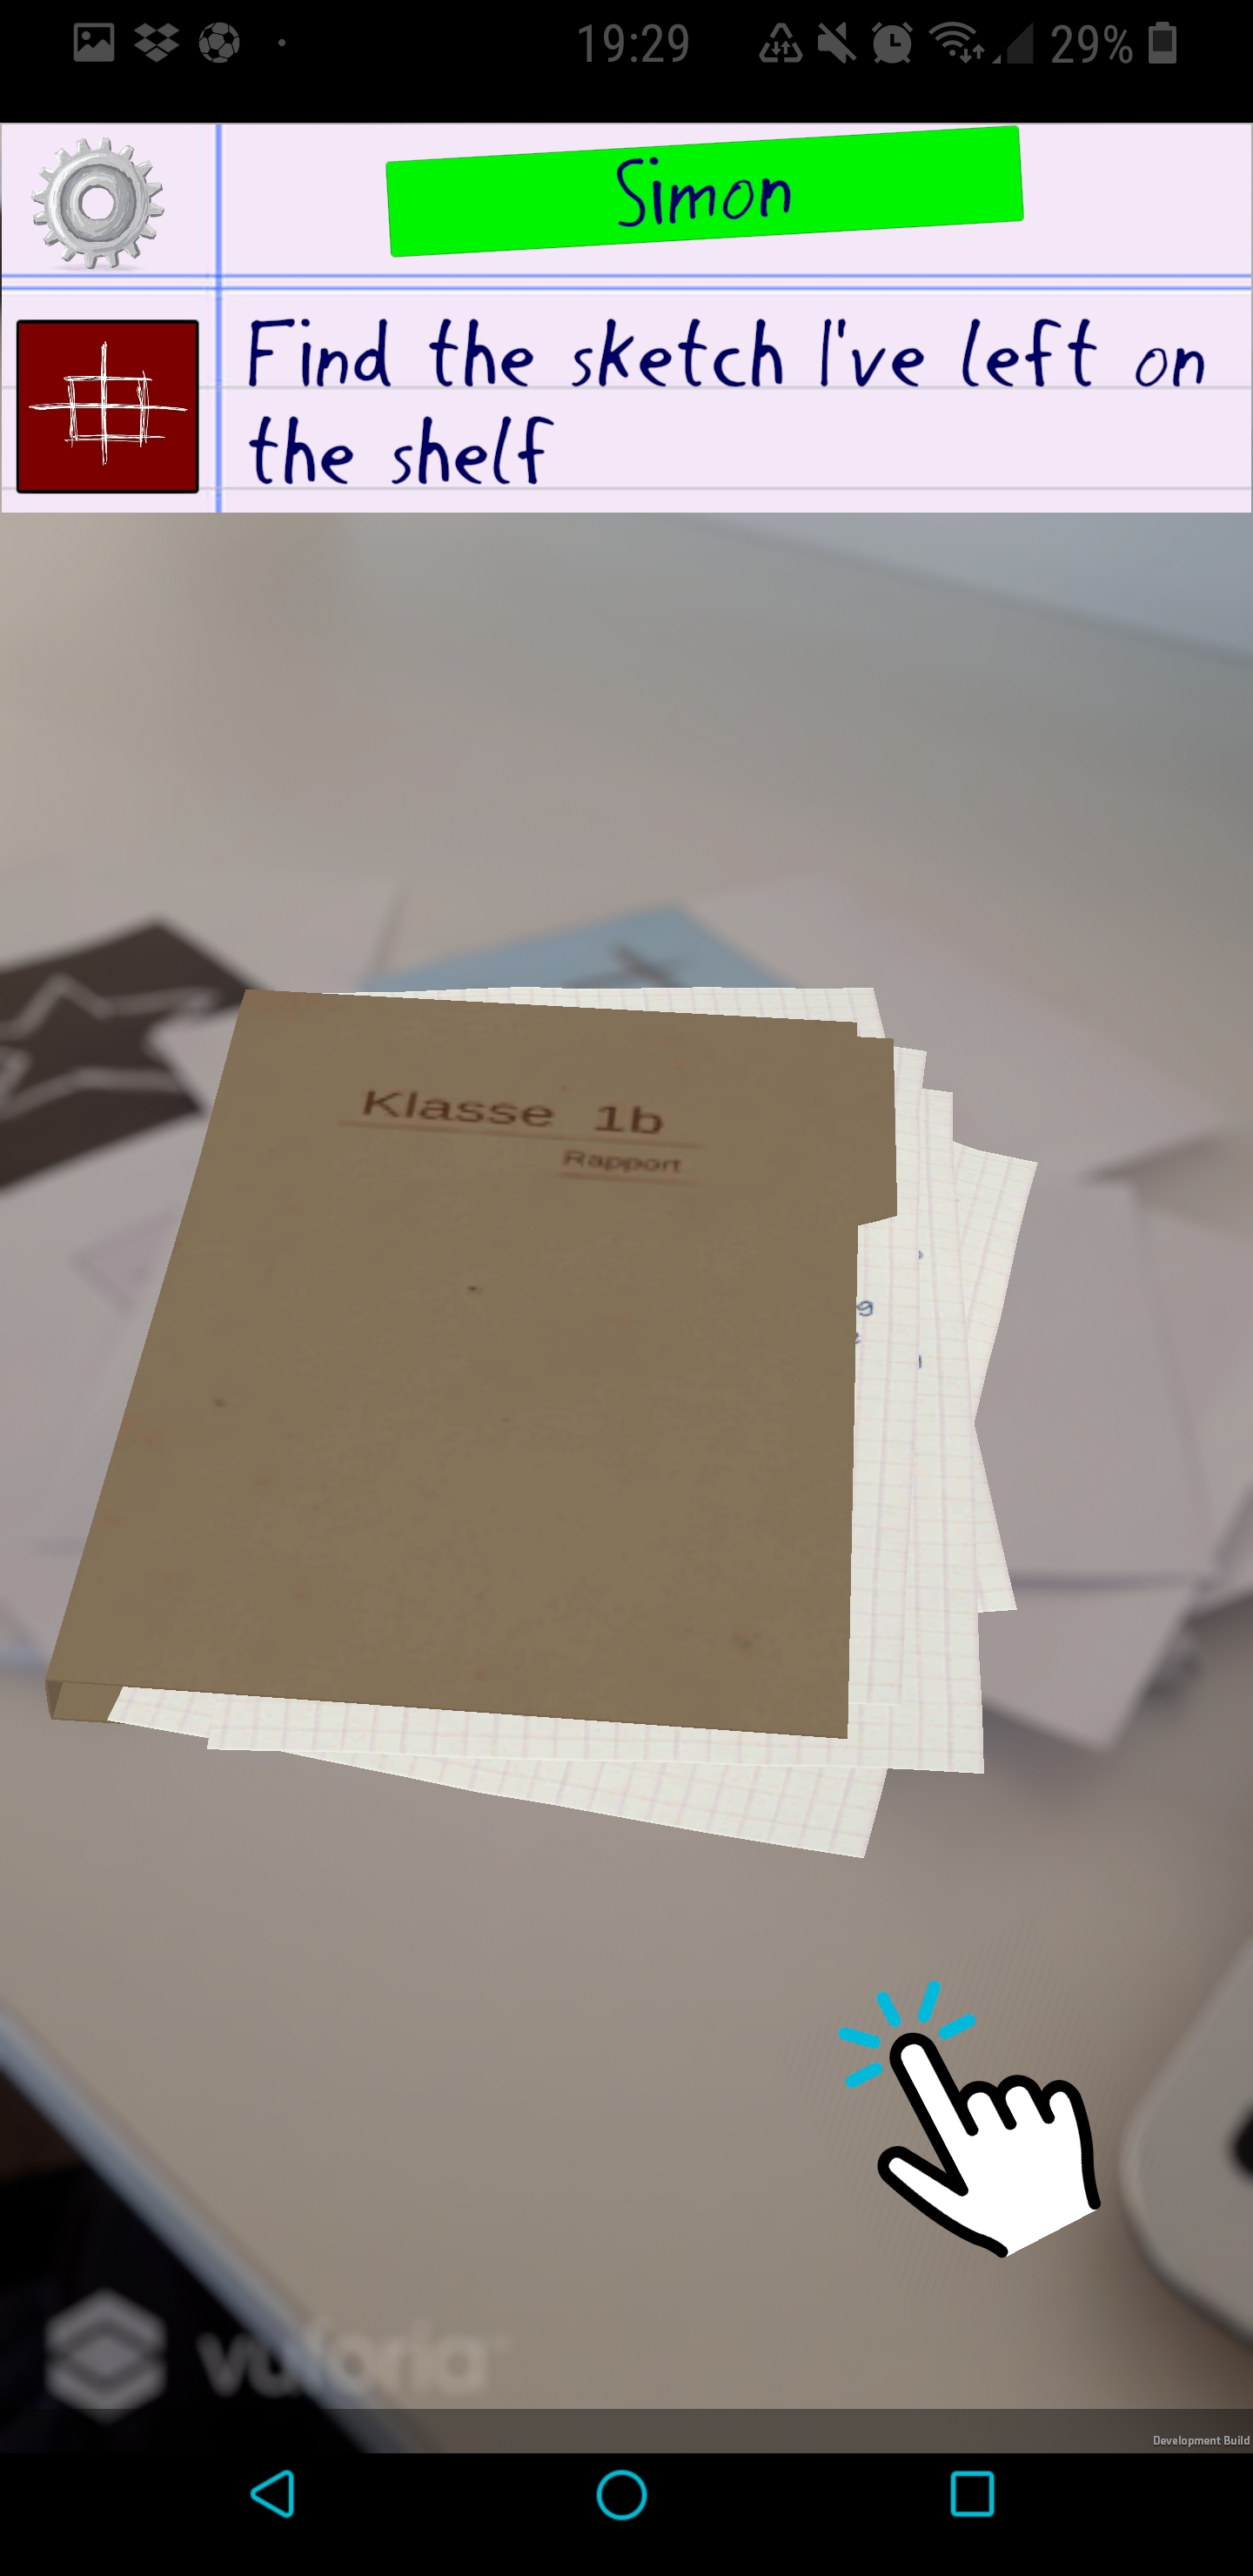
\includegraphics[scale = 0.07]{Screenshot_20190518-192941_LINA.jpg}
    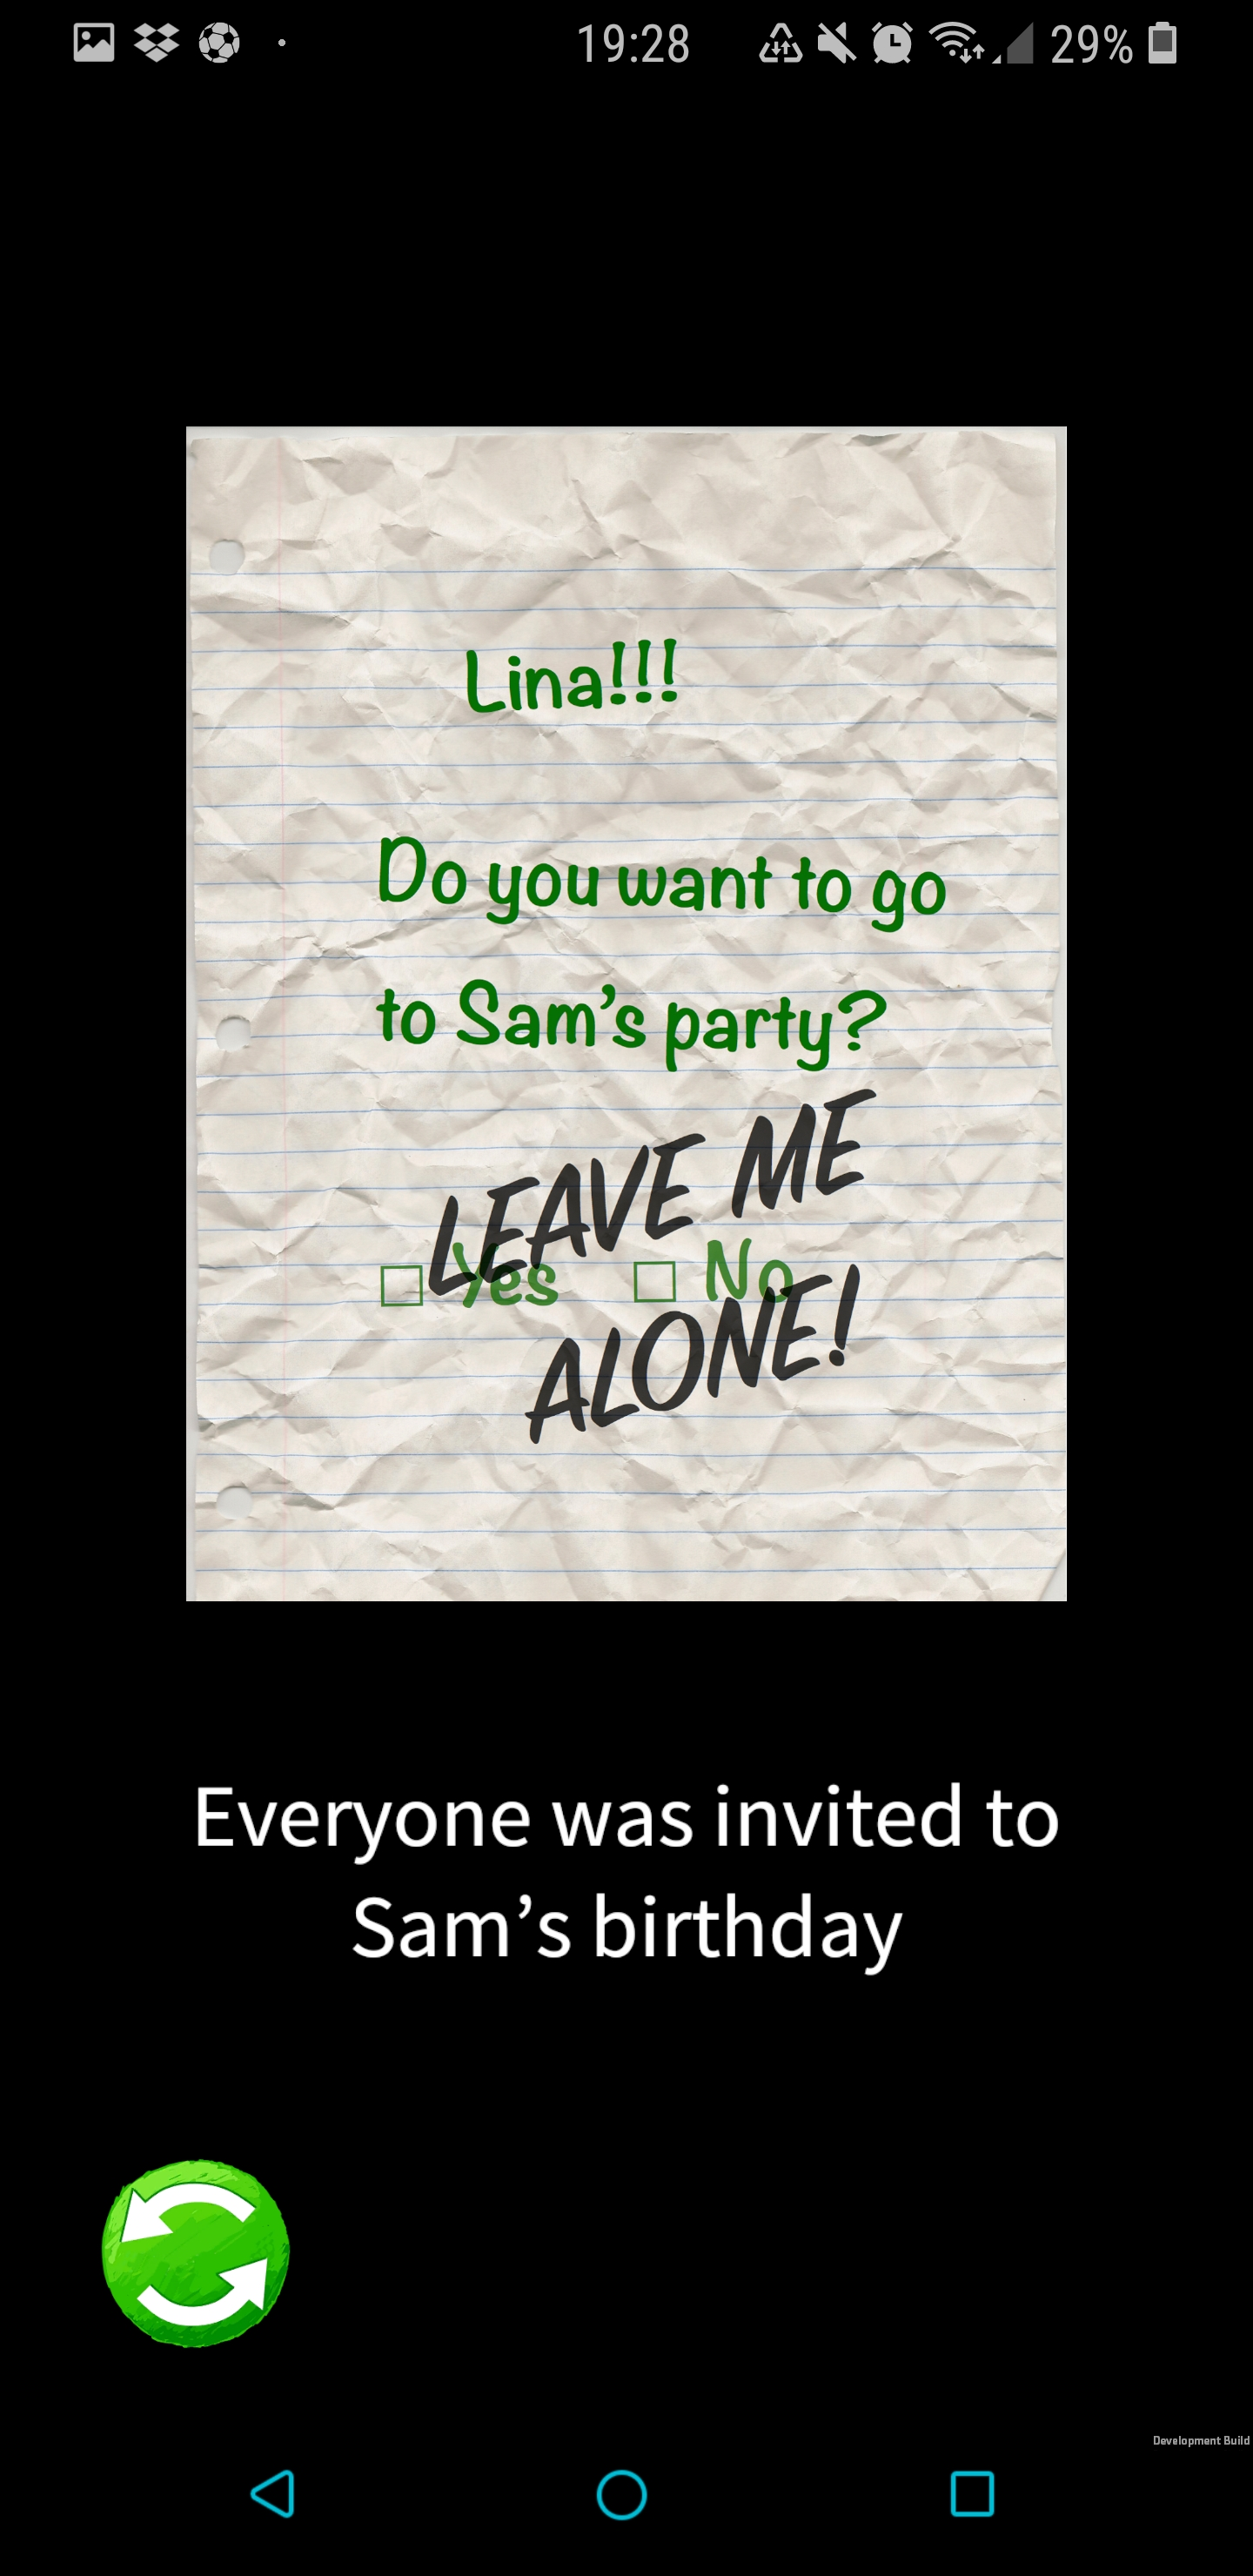
\includegraphics[scale = 0.07]{Screenshot_20190518-192847_LINA.jpg}
    \caption{These screenshots were taken from the second digital prototype: a) \textit{Exploration Mode}; b) \textit{View Mode}.}
    \label{fig:digital}
\end{figure}

\subsubsection{Usability}
\par In terms of usability, the game can be also divided in game modes: \textit{Exploration Mode}, \textit{View Mode}, and \textit{Interface Mode}. The player in each stage plays through one or more of these modes.
\par\textit{Exploration Mode} is the main scene in LINA, it is where the core mechanic of searching the world through imaging recovered live from the rear camera occurs. This was also the scene prone to more changes during the development. The recurring mechanic in a archetype 4 stage is: when the player scans a marker an augmented object appears, which the player needs to interact by tapping. Tapping that object usually unveils the real clue, and tapping on the clue usually triggers a narration and sends the player into \textit{View Mode}.
\par \textit{View Mode} is a screen where the players are shown an object relevant to the player. This was born out of the necessity of having a separate screen where the player could read an image containing text without having to keep the device scanning the marker. This screen also proves useful in presenting new objects that did not necessarily come from scanning a marker, for example, after the question challenge, when the new marker and instruction is unlocked.
\par \textit{Interface Mode} is any other scene where the player interacts with an interface, like when listening to its character narration or a in challenge. This usually follows the hand-script text on a notebook-style background, but not always: an example is the \textit{SMSApp} with its own style imitating a messaging application.

\subsubsection{Aesthetics}
\par In LINA there is a conscious effort to pass an immersive and atmospheric, almost cinematographic, feeling when playing the game. For that we made a number of decisions regarding the aesthetics: \textit{Exploration Mode} includes an atmospheric background music that accompanies the search for the markers, and sound effects when necessary. Also in "Exploration Mode", several post-processing filters like Grayscale, Sepia and Gaussian Blur were tested with the purpose of knowing the technical boundaries and what were the different cinematographic feelings conveyed. In particular, the Grayscale filter has been decided to be used in missions that are "flashbacks", being a typical visual effect used in media for that purpose; and the mixture of a blurred background and the sharp overlayed item provided a good effect aesthetically.
\par We also strive for realism with the markers and augmented reality clues, by trying to use realistic models. Pairing with the concept that art is Lina's best subject, the scribbled markers can become part of story, as if they were made by her, adding another layer of depth to the game. The design of the markers was changed in the middle of the development to fit the more realistic style [Fig.\ref{fig:icons}].
There is also a recurring art theme in the game: the hand-script on a notebook-style paper, as if the whole game was handwritten by Lina herself. This is further reinforced with an effort to have all interface images and buttons being drawings.
\par We also relied in established metaphors when designing the interface, not wanting it to be confusing and creating an obstacle that prevented the players from enjoying the experience: the "dented wheel" means settings, an arrow pointing right means "continue" and circular arrows mean "replay" (restarts the narration).

% #############################################################################

\subsection{Implementation}
The game was subject to several revision iterations, being developed first a low-fidelity prototype [Fig. \ref{fig:LFP}] from a supplied proof-of-concept document, then it was shown to experts and the playwright responsible for the narrative, iterated again, shown to the experts, and then developed a first version of the digital prototype, and then shown to the experts once more.
\par When designing the second prototype a design team was assembled, involving a playwright\cite{adam_barnard_2019} (tasked with designing the narrative) and a children psychologist, having weekly meetings regarding LINA and its design decisions. Due to time constraints it was not possible to have children testing the several prototype iterations, only the last one.

\begin{figure}
    \centering
    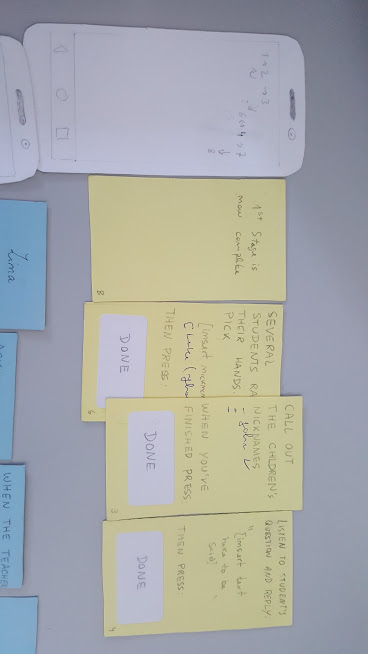
\includegraphics[scale = 0.3, angle = 90]{paper_proto1.jpg}
    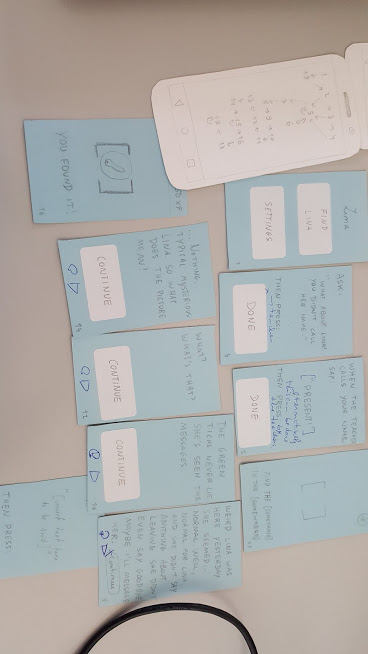
\includegraphics[scale = 0.3, angle = 90]{paper_proto2.jpg}
    \caption{Low-Fidelity Prototype of the teacher's and children's screen, respectively.}
    \label{fig:LFP}
\end{figure}

\subsubsection{Paper prototype} An initial low-fidelity paper prototype [Figs.\ref{fig:LFP}]was developed to conceptualize the interface and give some rough guidelines to fulfill the given script. A revision was made after presenting it to specialists where some suggestions regarding the presentation of some information texts and buttons.
\par The interface was chosen to be a simple area of text with some buttons on the bottom of the ``screen" (usually ``Back" and ``Next"), as to keep it simple, so that small children will not be distracted so easily, and to be intuitive, without ambiguities nor entropy. Blue and yellow colors seemed a very pleasant, non-intrusive and neutral background for the players and teacher, respectively.


\subsubsection{First digital prototype} The first digital prototype was made in the Unity3D Engine for its multi-platform support, and the Augmented Reality plug-ins that could be used to implement the scanning part. Initially, we thought that the markers could be QR codes to be scanned, however we decided to go directly for printed pictures instead, as the cost for implementation would be the same and there wasn't an advantage in starting with QR codes and changing to printed images later on.
\par For the Augmented Reality part we used \textit{Vuforia Augmented Reality SDK}, a plug-in that allows 2D or 3D ``markers" to be recognized and overlays an image or object in a position relative to the marker. The game uses a client-server approach to handle communication between the devices, as there must be a server app running as a game controller. This server also handles the synchronized communication used in the introduction, for example, where a dialogue scene must be coordinated between the teacher and his students. Contrary to the client apps, the server will be run in a computer.


\subsubsection{Second digital prototype} A second, and current, digital prototype [Fig.\ref{fig:digital}] was developed with the goal of presenting a minimal viable product for user testing. With this iteration we could experiment with the User Interface to see what would convey the feeling of the experience better - as it is supposed to have a realistic feeling, although a bit cartoon\textit{-ish}, due to Lina's drawings. Plus, some story was added and the cooperation parts were refined. 
\par For this prototype there was no need for a running server (as it was focused on the gameplay and the atmospheric feeling that was trying to be passed) so it was decided to make this version a local client where the user could choose between two "mock-up" players - Simon and Max - avoiding unnecessary complexity and the faults and could be derived from there. As the second prototype doesn't have a server and was just for showcasing purposes, the initial dialogue is skipped. Instead, there is an introduction video describing the initial exposition by the teacher.

% #############################################################################

\subsubsection{Changes Made for the Evaluation Workshop}

\par Some changes had to be made to the prototype for it to be properly played in the evaluation workshop. For instance, all text was translated to German. The note images that were written in English were left untouched, as was the audio narration, as there was not enough time to replace them for German translated ones and to be ready in time for the workshop.

	\section{Evaluation}
\label{sec:resul}

\subsection{Goals \& Workshop}
\par The purpose of the evaluation is to assess two things: how the children like the prototype in terms of enjoyment and satisfaction, i.e., whether they like the concept, have fun playing and want to play more; And the usability, whether the virtual and "real life" components of the game - interface and challenges - are adequate, and work well with each other, and individually.
\par To evaluate this, a workshop was conducted with children from a middle school in Austria. It consisted in two classes of children aged 10-12 years old, each class split in groups of 8 children. This was not always possible, so if needed one of us would fill in the role of the missing player. Each group had a session where they played as 4 different pairs - 4 play as Simon and the other 4 play Max - as if they were part of 4 different classes.  To decide who played as Simon and who played as Max, the children were seated in two rows of four: those in front would play as Max and those in the back play as Simon.
The markers were spread around the room before the workshop. Each session for a group took about 30 minutes, 5 for an introduction, 15 for the actual gameplay, and the remaining 10 to fill a quantitative questionnaire and have a little group discussion with some qualitative questions.
\par As the workshop was evaluating 4 pairs of players playing at the same time, new markers had to be created to accomodate that all those players. As Vuforia uses a grayscale image to recognize the pattern, new markers were devised with the same sketch but a different color, and a letter in the corner with the pair that belonged to (pair L,I,N, or A). However, Vuforia didn't properly distinguish the markers with the letters, so they become more indicative for the players than functional, as they could still scan a marker that "belonged" to another pair.

\subsection{Quantitative and Qualitative Instruments}

\par To evaluate the enjoyment/satisfaction and usability a quantitative questionnaire was constructed based on three scales: GSUS, an adapted version of SUS - System Usability Scale for game context \cite{molnar_kostkova_2014}, the Enjoyment subscale of GUESS - Game User Experience Satisfaction Scale \cite{phan_keebler_chaparro_2016} and the Interest/Enjoyment subscale of IMI - Intrinsic Motivation Inventory \cite{wilde_et_al_2009}. This questionnaire grouped some questions that were transversal to all three, and omitted others because it would take to long for the children to answer all the questions, plus some would not be suited for the children to answer, like the Usefulness subscale of IMI and GUESS. \par The answers were provided in a 5-point Likert scale with "thumbs up and down" images: "thumbs up" if they agreed with the statement, "thumbs down" if they disagreed. Also collected was their age, gender and class.

\par The focus interview followed a guide (based on the one from M Steiner et al. 2015)\cite{steiner_at_al_2015} with qualitative questions, also regarding enjoyment and usability, about their impression of the game and what they did and did not like in general, and two specific game components: the gameplay and the interface.

\subsection{Results}

\par These results were obtained from a population of 31 subjects - 13 males and 18 females, 9 being ten year-olds, 21 eleven year-olds and 1 thirteen year old - split in two classes: class 1A with 22 subjects - 10 males and 12 females - and class 1C with 9 subjects - 3 males and 6 females. 

\subsubsection{Quantitative Results}

\par These quantitative results come from the questionnaires answered after the play session. Cronbach's Alpha tests were conducted for each subscale to see if we could find a correlation between the questions that derived from the same subscale: the first six questions (derived from GSUS) and the other three (derived from IMI Interest/Enjoyment subscale and GUESS Enjoyment subscale). For this the results of questions 2 and 6 had to be inverted to the scale being inverted, i.e., lower score is better, while in the other questions, higher score is better. The results were 0.308 for the first six questions and 0.935 for the last three, which meant that questions 7-9 are directly correlated and could be treated as one, while 1-6 are independent. This could be due to the GSUS-based questions assessing several aspects of Usability, from playing difficulty to wanting to play more, which are not directly related. Henceforth questions 7-9 were grouped under the label "IMI\textunderscore Enjoyment".
\par First, from analyzing the given answers for each question [Fig.\ref{fig:Evaluation1}] the results are positive for both usability and interest/enjoyment, averaging the value of 4 out of 5 (also considering the inverted questions), which means that the inquired subjects agree with the following: 
\begin{itemize}
	\item They would like to play the game frequently;
	\item The game is not unnecessarily complex;
	\item The game was easy to play;
	\item The game does not have a steep learning curve;
	\item The players feel confident while playing the game;
	\item They did not need a lot of help to play the game;
	\item The game is fun;
	\item The game is interesting;
	\item They enjoyed playing the game;
\end{itemize}
\par A Chi-Square Test (all questions had p-value$<$0.05) refuted the hypothesis that the answers were the result of children randomly answering the questions. Then further checking the answers by splitting the population by gender and class [Fig.\ref{fig:Evaluation2}] revealed a notable gap in the mean values for some questions between the classes. This prompted conducting Mann-Whitney U Tests (p-value$<$0.05) to see if there was any relation between the answers and either gender and/or class. While its results showed no statistically significant difference regarding gender, the same cannot be said regarding class, for questions 1 (p=0.001), 5(p=0.014), 7(p=0.004), 8(p=0.004) and 9(p=0.004). This meant that class 1A, in comparison with 1C, enjoyed the game more and felt more confident while playing it, and subsequently would like more to play again in a frequently manner (although class 1C only has 9 subjects versus the 22 in 1A). This was first noticed during the feedback discussion at the workshop, and the collected data seems to confirm that perception. The second class was made up by "gifted" children, and it is curious to wonder why they enjoyed the game less or why they felt less confident while playing it. The psychologist hypothesized that, as overachievers, the children in that class were not comfortable with not understanding parts of the game and reacted more adversely than class 1A. Nevertheless, the overall usability and interest/enjoyment results were positive.
 
\subsubsection{Qualitative Results and Discussion}
\par This feedback results from the qualitative focus interview made after the children answered the questionnaire. Overall, the children liked the gameplay and the story. They wanted to play longer, and liked the challenges presented to them, but some did not work out as expected. Also, the interface worked well but there was some confusion regarding the narration, with the audio being in English and subtitles in German, that the players thought it was confusing.
\par They found the premise entertaining and fun; they also liked the question challenge, saying that this forced them to discuss the story. The image puzzle was not so well received by the class 1C, as they grew frustrated for not being able to finish the puzzle by themselves and had to effectively wait for the other player.
\par They did like the fact they are playing as fictional characters, but preferred having the option to choose their character's name, either from a list or submitting their own.
\par When asked to wait for the other player most would not do so and would just try every answer until he got the right one. This is a byproduct of this demo version as there isn't a server to check whether the player is really present or not. Afterwards the children explained that the instructions were confusing because they did not know if they were waiting for a real person or not and got inpatient waiting. Those that did wait criticized the waiting period, saying it took to long for the other player to get there. Nonetheless, they praised the cooperation with their colleagues, specially with having to pair with a random person and not only with their best friend.  
\par Regarding the interface they thought it was quite clear, but some were confused and did not know what they were supposed to do in \textit{Exploration Mode} and instead of scanning the markers, started scanning the whole room to see if something happened. Some, when scanned their first marker, did not understand that were supposed to tap on the augmented object.

\begin{figure}
	\centering
	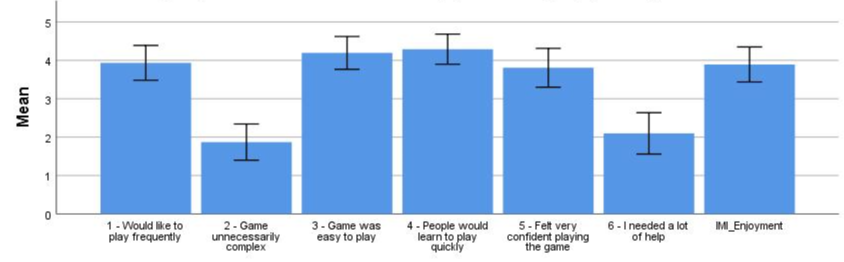
\includegraphics[scale = 0.35]{Mean.png}
	\caption{The mean results of the questionnaire, with a 95\% Confidence Interval. For questions 2 and 6, lower is better.}
	\label{fig:Evaluation1}
\end{figure}

\begin{figure}
	\centering
	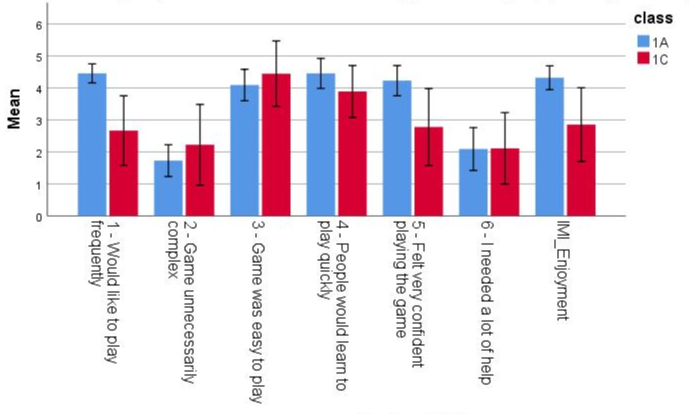
\includegraphics[scale = 0.4]{MeanPerClass.png}
	\caption{The mean results of the questionnaire per class, with a 95\% Confidence Interval. For questions 2 and 6, lower is better.}
	\label{fig:Evaluation2}
\end{figure}




	\section{Conclusions}
\label{sec:concl}
\par An initial prototype for a cooperative Augmented Reality mobile game was presented, with the goal of improving relations between classmates, based on Contact Theory. This game consists in having a sort of interactive theater play, directed by the game, to find what happened to a colleague of theirs through the search of Augmented Reality clues and challenges to be completed through teamwork. Three iterations were made: a paper prototype, a basic technical proof-of-concept involving a server, and a second prototype, more focused on the User Interaction and the challenges proposed to the players.
\par A workshop was conducted to evaluate the Usability and Enjoyment of the prototype through a quantitative questionnaire based on the System Usability Scale, Intrinsic Motivation Inventory, and Game User Experience Satisfaction Scale questionnaires, plus an interview for qualitative feedback. This workshop had some interesting findings and, as it was the first time the game was played by the actual target group, was extremely useful for observing their natural reaction to the whole premise, interface, and challenges proposed. It was successful in two ways: first, it showed that the children are interested and would enjoy playing LINA, and second, it showed that not only is the prototype almost totally usable, but also pointed out what aspects to improve for that end. 
\par With the feedback from the session, future work will consist in improving some aspects of this prototype, while also looking at new challenges and exploring further the technological limits of Augmented Reality in the context of this game.

% REFERENCES

% Produces the bibliography section when processed by BibTeX
%
% Bibliography style
% > entries ordered alphabetically
%\bibliographystyle{plain}
% > unsorted with entries appearing in the order in which the citations appear.
%\bibliographystyle{unsrt}
% > entries ordered alphabetically, with first names and names of journals and months abbreviated
\bibliographystyle{abbrv}
% > entries ordered alphabetically, with reference markers based on authors' initials and publication year
%\bibliographystyle{alpha}

% External bibliography database file in the BibTeX format (ExtendedAbstract_ref_db.bib)
\bibliography{references}

\end{document}


